\section{Background}
For a unified RDMA virtualization in hybrid virtual environments, we should note the differences between VMs and containers, the virtualiztion methods for I/O device and the RDMA network. Thus, we introduce a brief background about above in this section.

\subsection{Virtualization}
Virtualization of VMs and containers are in different spaces because of their characteristics. VMs need emulate whole virtual hardware environments for guest operation system with hypervisor (kernel-space). So, applications in VMs is isolated by guest OS with more security but higher overhead. Containers are shared with the host OS but with runtime isolation. So, containers have low overhead and fast boot-up time.

For software virtualization of I/O devices, there are two main choices for where to emulate the device: kernel-space and user-space. In kernel-space, the codes of device emulation are inserted into hypervisor or host kernel. Compared to kernel-space, there are three advantages for user-space: first, the attack surface is limited for user-space with minimal inserted code into kernel/hypervisor; second, managment development is flexible in user-space; third, the inserted codes are often depenedent on hardware-specific APIs (e.g. OS architecture, device driver). For example, vhost-net~\cite{vhost-net} is the kernel-space network device and vhost-user-net~\cite{vhost-user-net} has user-mode virtual device. 


% RDMA: 
% RDMA网卡是控制和数据路径分离, RDMA网卡内部构造
% RDMA网卡数据传输机制,按门铃操作
\subsection{RDMA}
RDMA (Remote Direct Memory Access) has hardware protocol stack and zero copy technology, so applications can bypass the kernel to read and write remote memory data, without the participation of remote CPU. As a result, RDMA has high throughput, low latency and low CPU load. Applications need to use Verbs interface when using RDMA. In Verbs, as shown in Figure~\ref{fig:rdma-feat}, RDMA is separate control path and data path. The former is the management about RDMA context, mainly including lots of RDMA resources, such as Queue Pairs (QPs), and Memory Regions (MRs). the operations like ibv\_create\_qp, reg\_mr; The latter is the usage of RDMA context and resources, which is the data commands like ibv\_post\_send and ibv\_post\_recv. In a RDMA workflow, the communication is based on Queue Pair (QP). The application writes the RDMA work request to the QP, and then ``press''  the RNIC's doorbell register, which is mapped to application when context init, and the RNIC's hardware processor will execute the work request in the QP to forward data. For applications, the entire operator is in the user space.


\begin{figure}[!ht]
	\centering
	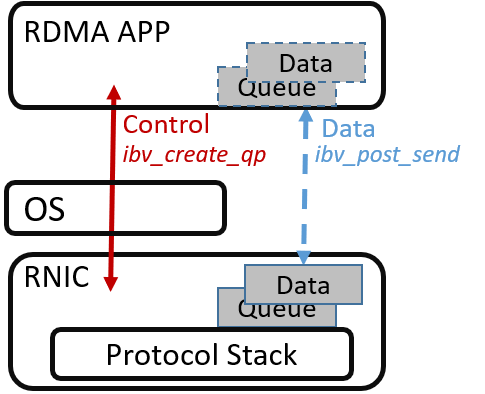
\includegraphics[width=0.6\linewidth]{images/rdma-feat.png}
	\caption{Native RDMA Feature}
	\label{fig:rdma-feat}
\end{figure}


